\graphicspath{{05-EMR/Figures/}}

\section{Electron Muon Ranger}
\label{Sect:EMR}

\subsection{Introduction}
\label{SubSect:EMR_Intro}

The Electron-Muon Ranger (EMR) is a fully-active scintillator detector~\cite{2016JInst..11T10007}. It can be classified as a tracking-calorimeter as its granularity allows for track reconstruction. The EMR consists of extruded triangular scintillator bars arranged in planes. One plane contains 59 bars and covers an area of 1.27\,m$^2$. Each even bar is rotated by 180 degrees with respect to the odd one. A cross-section of bars and their arrangement in a plane is shown in Fig.~\ref{fig:EMR}. This configuration does not leave dead area in the detector for particles crossing a plane with angles that do not exceed 45 degrees with respect to the beam axis. Each plane is rotated through 90 degrees with respect to the previous one, such that a pair of planes defines a horizontal and vertical $(x, y)$ interaction coordinate. The light, produced when a particle crosses a bar, is collected by a wave-length shifting (WLS) fibre glued inside the bar. At both ends, the WLS fibre is coupled to clear fibres that transport the light to a photomultiplier tube (PMT). Signals produced in a plane are read out collectively on one end by a single-anode PMT for an integrated charge measurement and separately on the other by a multi-anode PMTs for individual bar hit reconstruction. The full detector is composed of 24 X--Y modules for a total active volume of $\sim 1$\,m$^3$.

\begin{figure}
	\begin{center}
		\includegraphics[width=0.465\columnwidth]{EMR1.png}
		\hfill
		\includegraphics[width=0.515\columnwidth]{EMR2.jpg}
		\caption{Drawing of one EMR plane (top left), cross section of 3 bars and their wavelength shifting fibres (bottom left) and drawing of the full detector (right).}
		\label{fig:EMR}
	\end{center}
\end{figure}

An array of analyses were conducted to characterize the hardware of the EMR and determine whether the detector performs to specifications~\cite{Drielsma:2017doj}. The clear fibres coming from the bars were shown to transmit the desired amount of light, and only four dead channels were identified in the electronics. Two channels had indubitably been mismatched during assembly and the DAQ channel map was subsequently corrected. The level of crosstalk is within acceptable values for the type of multi-anode photomultiplier used with an average of $0.20\pm0.03$\,\% probability of occurrence in adjacent channels and a mean amplitude equivalent to $4.5\pm0.1$\,\% of the primary signal intensity. The efficiency of the signal acquisition, defined as the probability of recording a signal in a plane when a particle goes through it in beam conditions, reached $99.73\pm0.02$\,\%.

The primary purpose of the EMR is to distinguish between muons and their decay products, identifying
muons that have crossed the entire cooling channel. Muons and electrons exhibit distinct behaviours in the detector. A muon follows a single straight track before either stopping or exiting the scintillating volume, while electrons shower in the lead of the KL and create a broad cascade of secondary particles. Two main geometric variables, the plane density and the shower spread, are used to differentiate them. The detector is capable of identifying electrons with an efficiency of 98.6\,\%, providing a purity for the MICE beam that exceeds 99.8\,\%. The EMR also proved to be a powerful tool for the reconstruction of muon momenta in the range 100--280\,MeV/$c$~\cite{2015JInst..10P2012A}.

\subsection{Performance}
\label{SubSect:EMR_Performance}

\subsubsection{Efficiencies}
The data sets used to evaluate the detector efficiencies are summarized in table~\ref{tab:emr_eff_data_sets}. The MICE beam line is tuned to the highest attainable momentum to maximize the transmission to the EMR detector and increase the range of particles in the detector. In this configuration, the beam line produces pions and muons in comparable quantities, along with positrons. The particle species are identified by evaluating their time-of-flight between TOF1 and TOF2. The time-of-flight distribution for muons, pions and positrons is represented in figure~\ref{fig:emr_eff_tof}. Only the particles with a time-of-flight between 28 and 28.75\,ns, i.e. compatible with the muon hypothesis, are included in the analysis sample.

\begin{table}
	\centering
	\begin{tabular}{c|c|c|c|c|c|c}
		Run ID & Date & Type & Momentum & Spills & Triggers & EMR events \\
		\hline
		9619 & 19/09/2017 & $\pi^+$ & 400 MeV/$c$ & 2289 & 265312 & (\textcolor{red}{to do}) \\
		9620 & 19/09/2017 & $\pi^+$ & 400 MeV/$c$ & 5388 & 668026 & (\textcolor{red}{to do}) \\
		\hline
		\multicolumn{3}{c}{} & \textbf{Total} &  &  & 
	\end{tabular}
	\caption{Summary of the data sets used to measure the efficiency of the EMR in the 2017/02 ISIS user cycle.}
	\label{tab:emr_eff_data_sets}
\end{table}

    \begin{figure}
    	\begin{center}
    		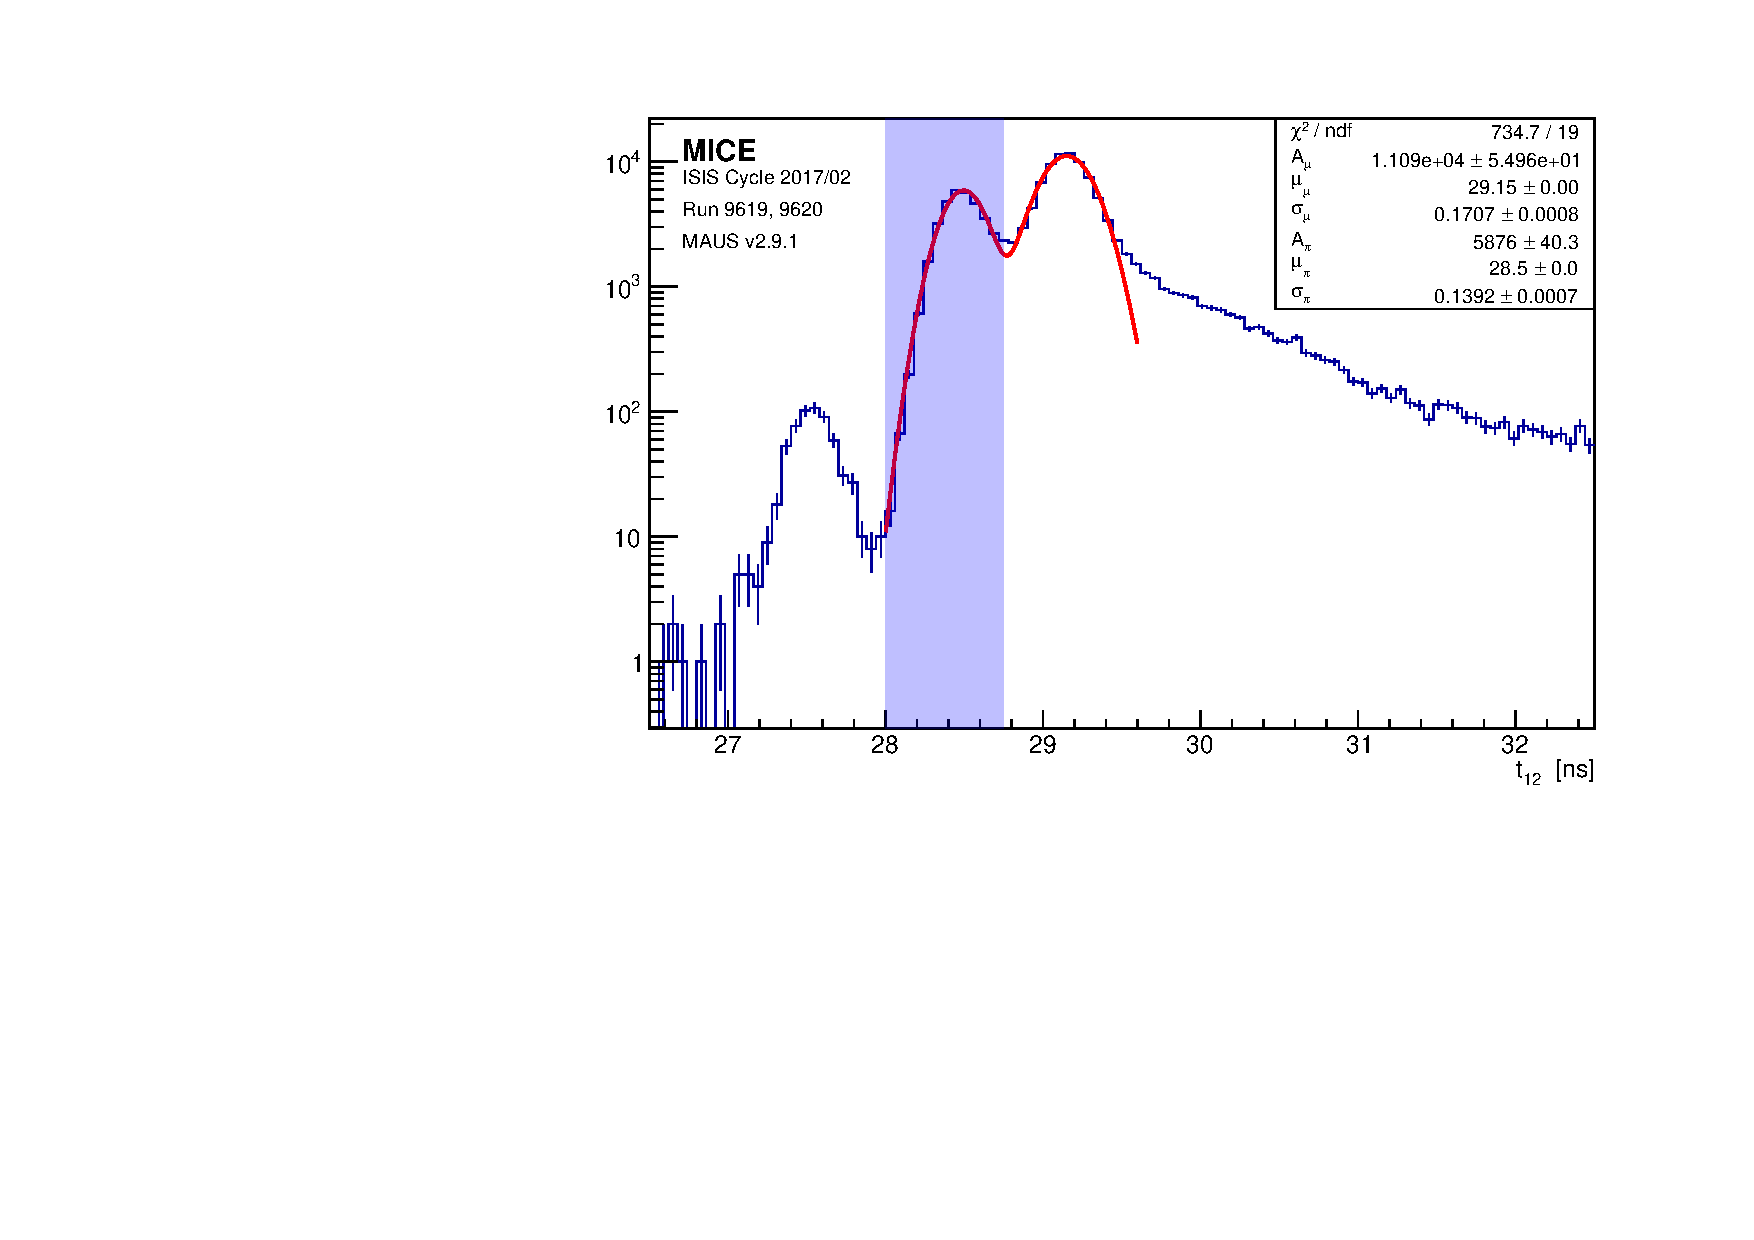
\includegraphics[width=0.6\columnwidth]{tof12.pdf}  		
    		\caption{Time-of-flight of positrons, muons and pions for the 400\,MeV/$c$ pionic beam line used in the EMR efficiency analysis. The blue band represents the selected range.}
    		\label{fig:emr_eff_tof}
    	\end{center}
    \end{figure}

A muon that makes it into the analysis sample has a momentum larger than 350\,MeV/$c$ right before TOF2. It is expected to cross both TOF2 and the KL without stopping and penetrate the EMR. In practice, the probability of creating an EMR event, i.e. to produce hits in the detector is $99.67\pm0.06\,\%$. The minor inefficiency may be attributed to pions in the muon sample that experience hadronic interactions in the KL. If hits are produced in the detector, space points are reconstructed $98.82\pm0.12\,\%$. This inefficiency may be associated with muon that decay between TOF2 and the EMR and produce scarce hits in the detector (\textcolor{red}{to update}).

To evaluate the efficiency of the scintillator planes and their readouts, only the muons which penetrate the entire detector are taken into account. If a signal is recorded in the most downstream plane, it is expected that at least a bar will be hit in each plane on its path and that a signal will be recorded in the single anode PMT. The left panel of figure~\ref{fig:emr_eff} shows the MAPMT bar hit multiplicity for all the plane combined. It shows that in $3.00\pm0.00\,\%$ (\textcolor{red}{to do}) of cases, on average, a plane traversed by a muon will be not produce a signal in its MAPMT and that the most probable amount of bars hit is one. The right panel shows the distribution of charge recorded in the all the SAPMTs. A track is missed by an SAPMT $0.15\pm0.00\,\%$ (\textcolor{red}{to do}) of the time.

\begin{figure}
	\begin{center}
		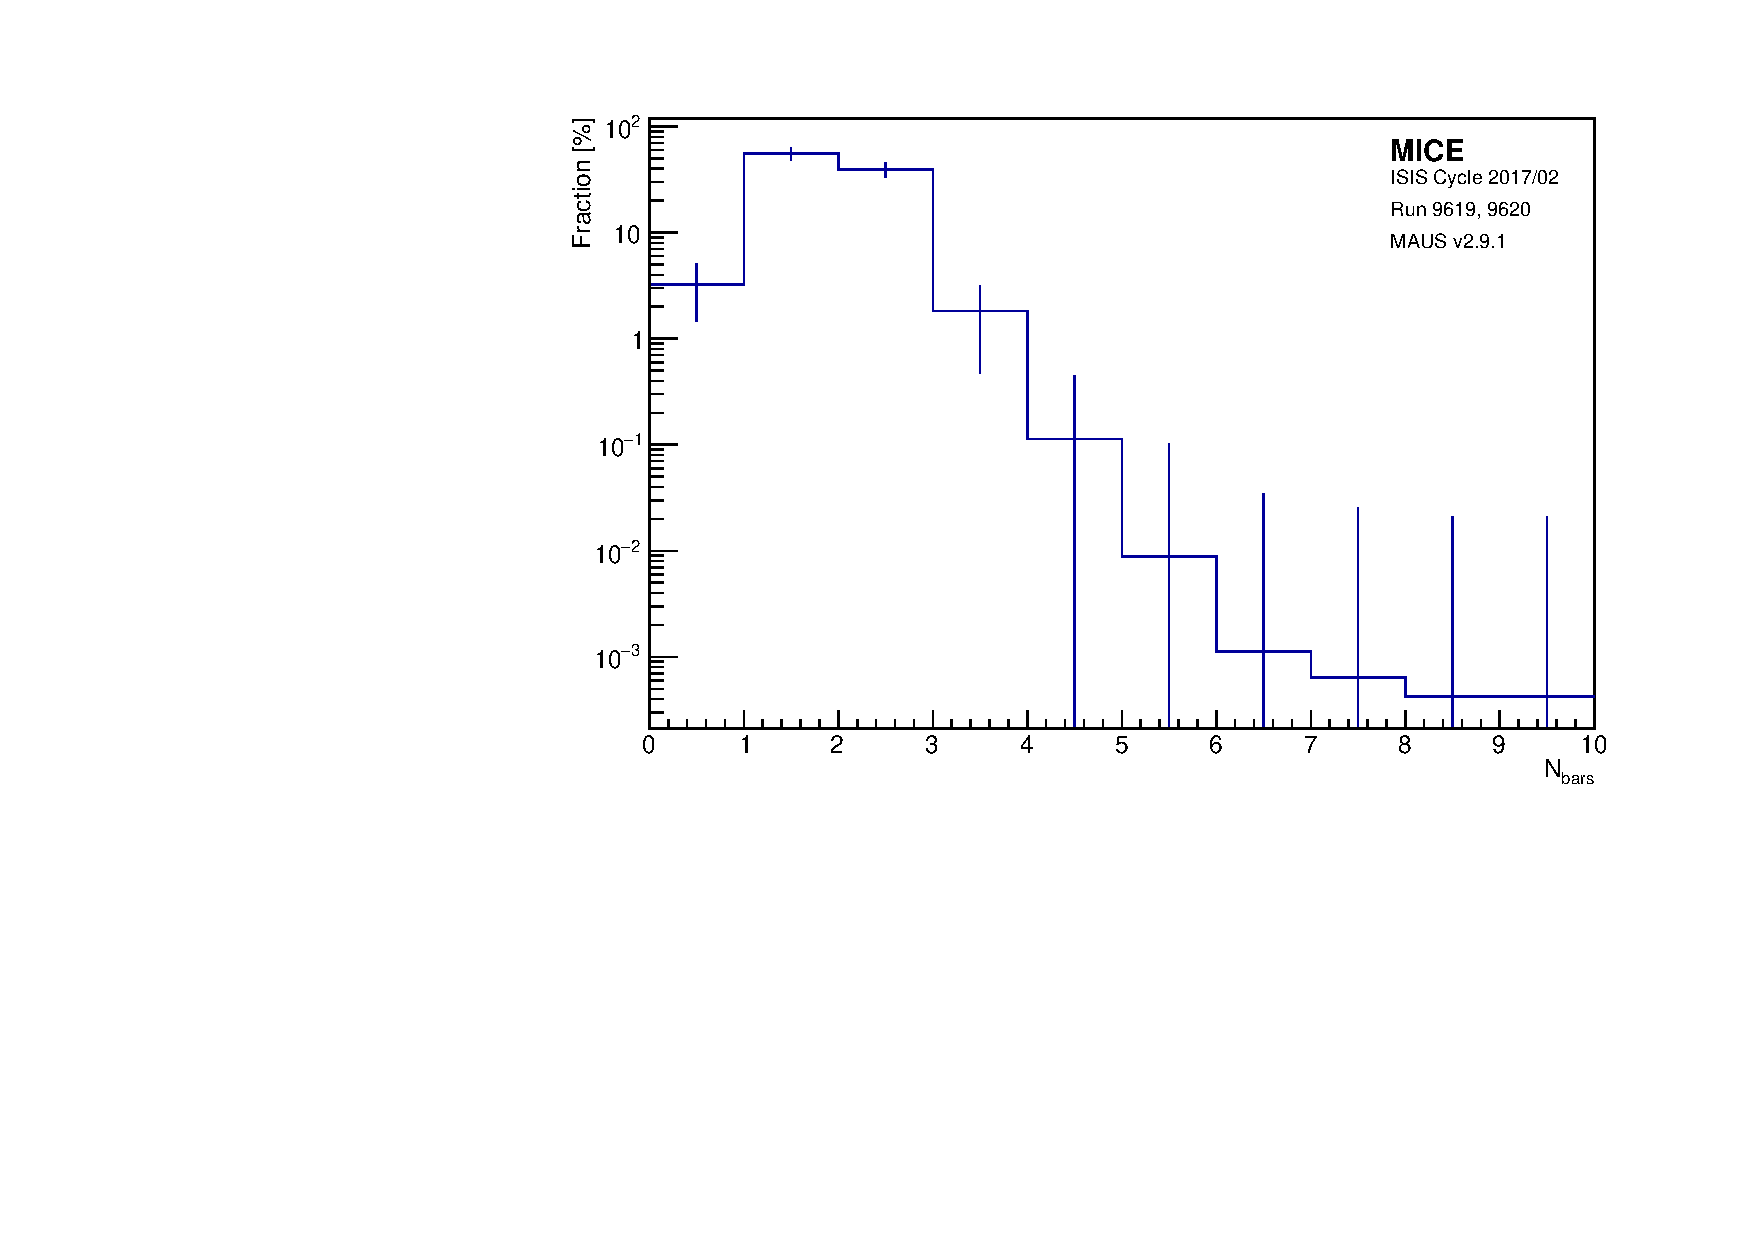
\includegraphics[width=0.49\columnwidth]{nbars.pdf}
		\hfill
		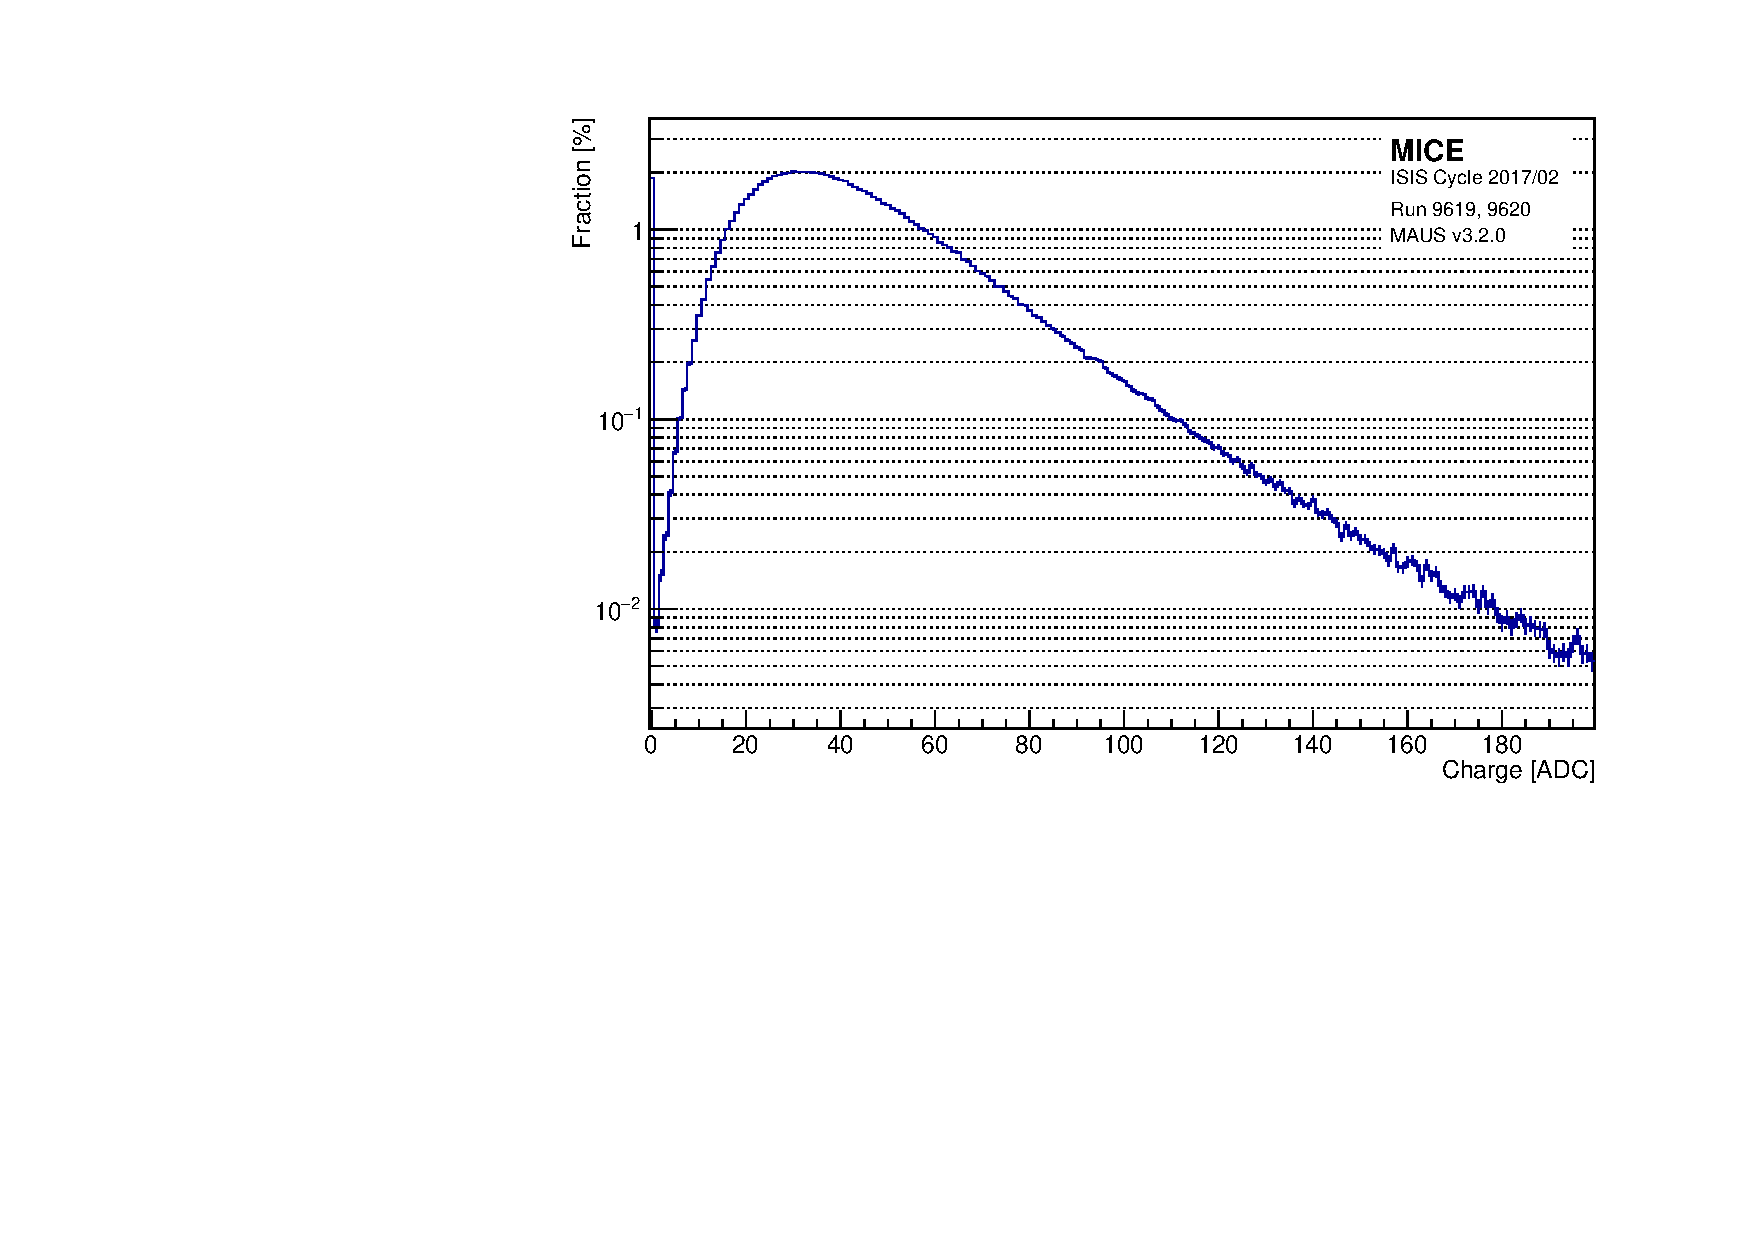
\includegraphics[width=0.49\columnwidth]{charge.pdf}
		\caption{(Left) Average MAPMT bar multiplicity. (Right) Average SAPMT charge distribution.}
		\label{fig:emr_eff}
	\end{center}
\end{figure}

Figure~\ref{fig:emr_plane_eff} shows the probability of recording a signal in individual MAPMTs and the SAPMTs for each of the 48 planes, given a muon that crosses the whole detector. The most inefficient PMTs miss the track $\sim10\,\%$ of the time. SAPMT 26 was experiencing issues during data taking and was turned off.

\begin{figure}
	\begin{center}
		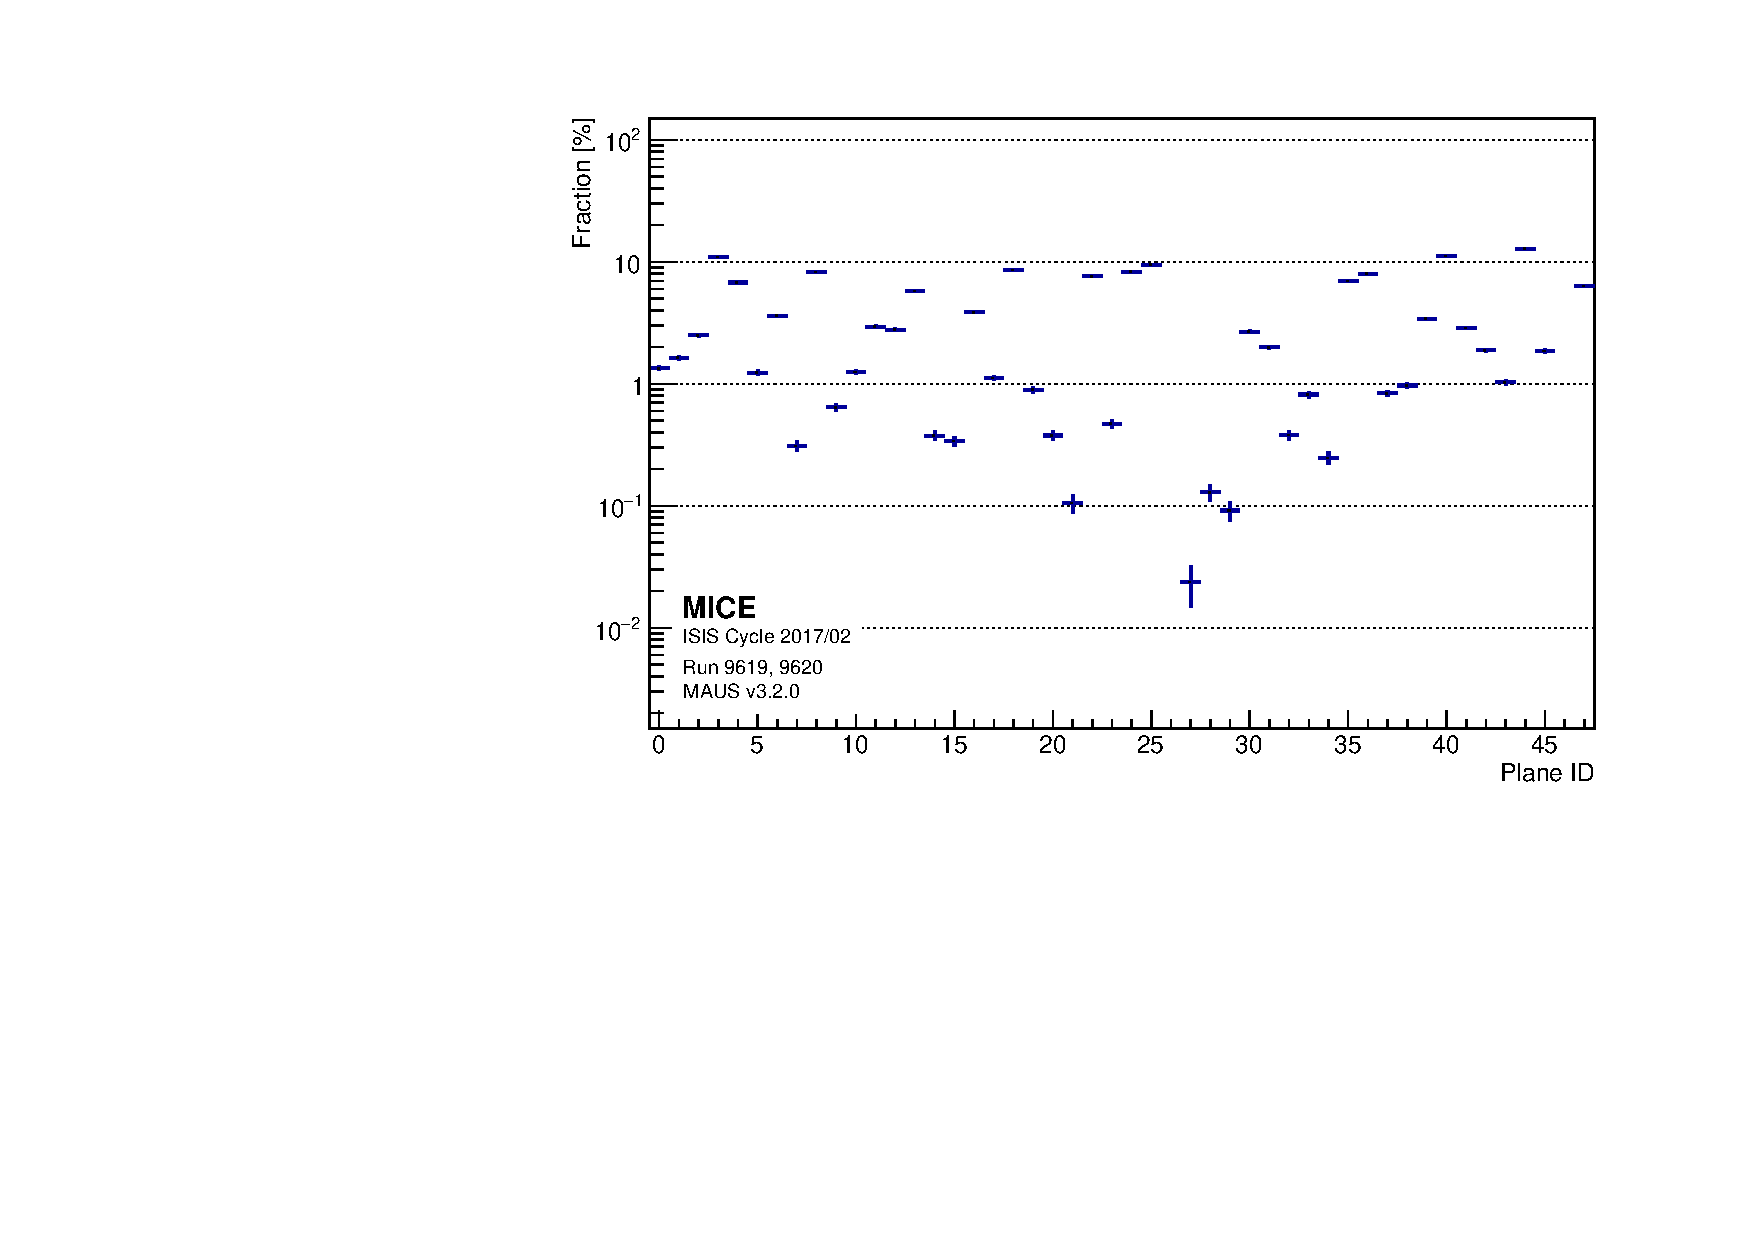
\includegraphics[width=0.49\columnwidth]{missed_mapmt.pdf}
		\hfill
		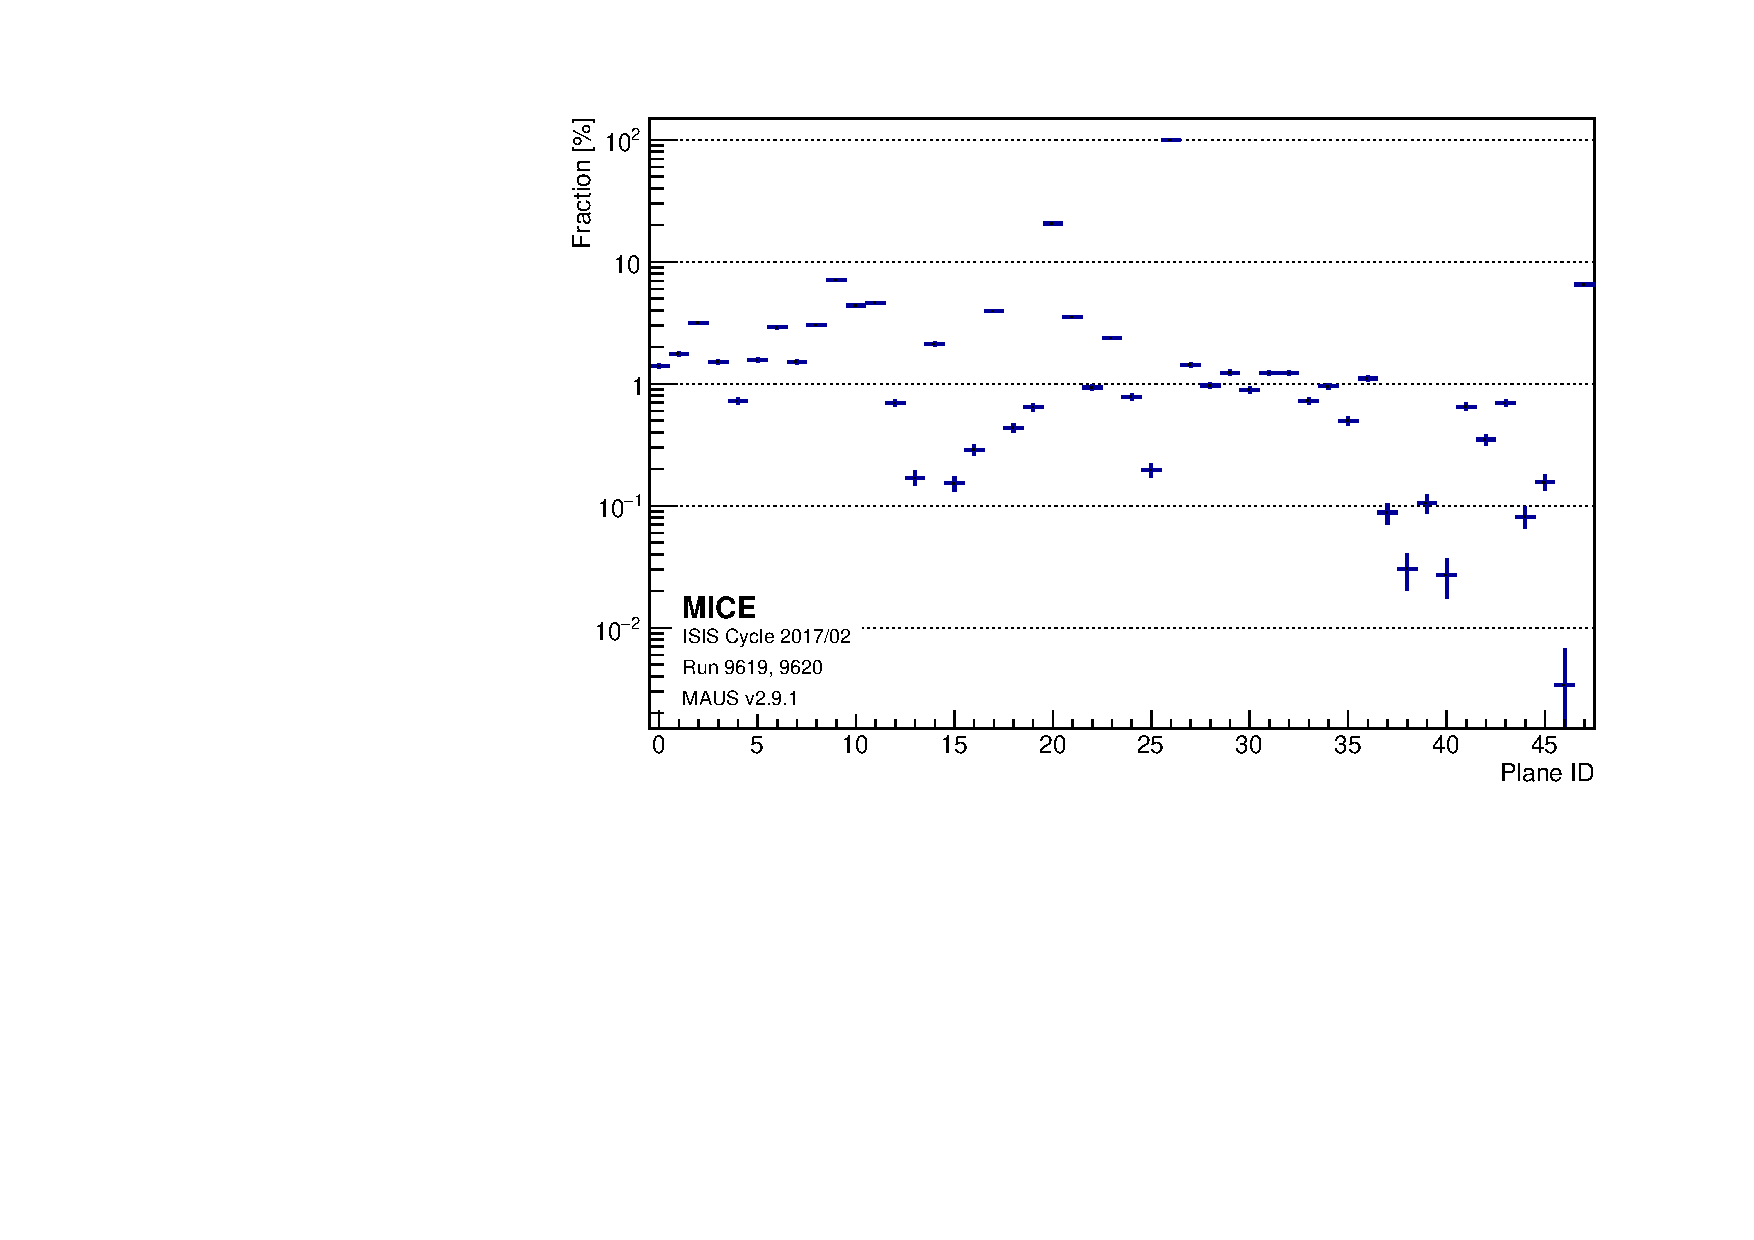
\includegraphics[width=0.49\columnwidth]{missed_sapmt.pdf}
		\caption{Probability of producing at least a single bar hit in the MAPMT (left) and a non-zero charge in the SAPMT (right) in the 48 individual EMR planes.}
		\label{fig:emr_plane_eff}
	\end{center}
\end{figure}

\subsubsection{Reconstruction}
\begin{itemize}
	\item Show a muon + an electron event;
	\item Show the muon range for different sets of input momentum;
	\item Show the muon angular distributions + beam profile;
	\item Show the muon momentum reconstructed, as a function of impinging momentum (for TKD?).
\end{itemize}

\subsubsection{Electron rejection}

\begin{itemize}
	\item Show the plane density profiles (e+mu);
	\item Show the $\chi^2$/ndf (e+mu);
	\begin{equation}
	\hat{\chi}^2=\frac{1}{N-4}\sum_{i=1}^{N}\frac{\text{res}_{x,i}^2+\text{res}_{y,i}^2}{\sigma_x^2+\sigma_y^2}
	\end{equation}
	\item Compute the contamination;
	\item Repeat for multiple momenta (200, 240, 170?, 140 futile).
\end{itemize}

